% Settings for the default beamer theme
\documentclass[english, aspectratio=169]{beamer}
\usepackage{babel}
\usepackage{tabularx}
\usepackage[T1]{fontenc}
\usepackage[utf8]{inputenc}
\setcounter{secnumdepth}{3}
\setcounter{tocdepth}{3}

\makeatletter

\newcommand\makebeamertitle{\frame{\maketitle}}

% (ERT) argument for the TOC
\AtBeginDocument{%
  \let\origtableofcontents=\tableofcontents
  \def\tableofcontents{\@ifnextchar[{\origtableofcontents}{\gobbletableofcontents}}
  \def\gobbletableofcontents#1{\origtableofcontents}
}

% Theme settings
\usetheme{Frankfurt}
\usecolortheme{default}
\usefonttheme[onlymath]{serif}

% Template settings
\setbeamertemplate{navigation symbols}{}
\setbeamertemplate{blocks}[rounded][shadow=false]
\setbeamertemplate{title page}[default][colsep=-4bp, rounded=true, shadow=false]
\makeatother

\begin{document}

% Title page
\section{Bevezetés}
\title[]{Üzleti Intelligencia}
\subtitle{3. Előadás: Markov döntési folyamatok megoldása}
\author[Kuknyó Dániel]{Kuknyó Dániel\\Budapesti Gazdasági Egyetem}
\date{2023/24\\1.félév}
\makebeamertitle

% Table of contents slide
\begin{frame}
\tableofcontents{}
\end{frame}

% Table of contents of the current section
\begin{frame}
\tableofcontents[currentsection]
\end{frame}

\begin{frame}{Az RL modellje}
\begin{columns}
\begin{column}{.5\textwidth}
\only<1>{\begin{block}{Markov döntési folyamat}
\[
\left(S,A,P,R,s_{0},\gamma\right)
\]
\begin{itemize}
	\item $S$: állapotok halmaza
	\item $A$: cselekvések halmaza
	\item $P:\; S \times A \times S \rightarrow [0,1]$: állapotátmeneti valószínűségek
	\item $R:\; S \times A \rightarrow \mathbb{R}$: azonnali jutalmak halmaza
	\item $s_{0}$: kezdőállapot
	\item $\gamma$: diszkont faktor
\end{itemize}
\end{block}}
\only<2>{Az MDP folyamata:\\
\begin{enumerate}
	\item Az ügynök $s_{0}$ állapotból indul
	\item Az ügynök $\pi$ politika szerint cselekszik: $a_{t}\sim\pi(s_{t})$
	\item A környezet reagál a cselekvésre, és visszaadja az ügynöknek $r_{t+1}$ jutalmat és $s_{t+1}$ következő állapotot
	\item Ez ismétlődik amíg a kilépési kritérium be nem teljesül
\end{enumerate}
Cél: Az optimális politika megtalálása. A politika optimális, ha a hozamának várható értéke maximális:
\[
E_{\pi}\left(r_{1} + \gamma r_{2} + \gamma^{2}r_{3} + ...\right) \rightarrow max
\]}
\end{column}
\begin{column}{.5\textwidth}
\begin{center}
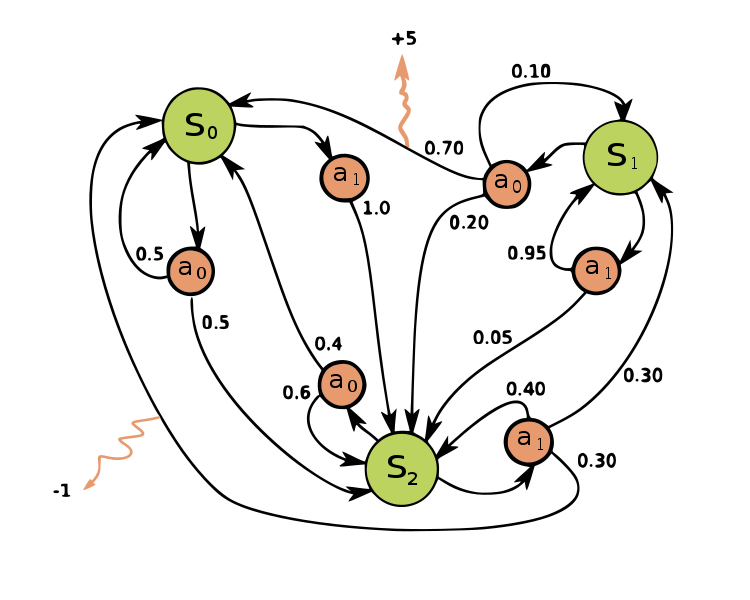
\includegraphics[width=7cm, height=7cm, keepaspectratio]{images/solving_1.png}
\end{center}
\end{column}
\end{columns}
\end{frame}

\begin{frame}{A mohó ügynök}
\begin{columns}[T]
\begin{column}{.5\textwidth}
A legegyszerűbb cselekvés kiválasztási szabály, ha az ügynök mindig azt a cselekvést választja, ami számára a lehető legnagyobb várható hozammal rendelkezik.
\begin{center}
\begin{block}{Mohó cselekvés választás}
Mohó politika mindig azt a cselekvést fogja választani, amelyik - egy lépéses távlatban - a lehető legnagyobb várható jutalommal fog járni az ügynök számára $v_{\pi}$ szerint.
\[
A_{t}=\underset{a}{argmax}\:Q_{t}(a)
\]
\end{block}
\end{center}
\end{column}
\begin{column}{.5\textwidth}
\begin{itemize}
	\item Mi lenne a mohó politika ebben az estben?
	\item Mindig ez a legjobb megoldás?
	\item A legjobb megoldás mindig mohó?
\end{itemize}
\begin{center}
\only<1>{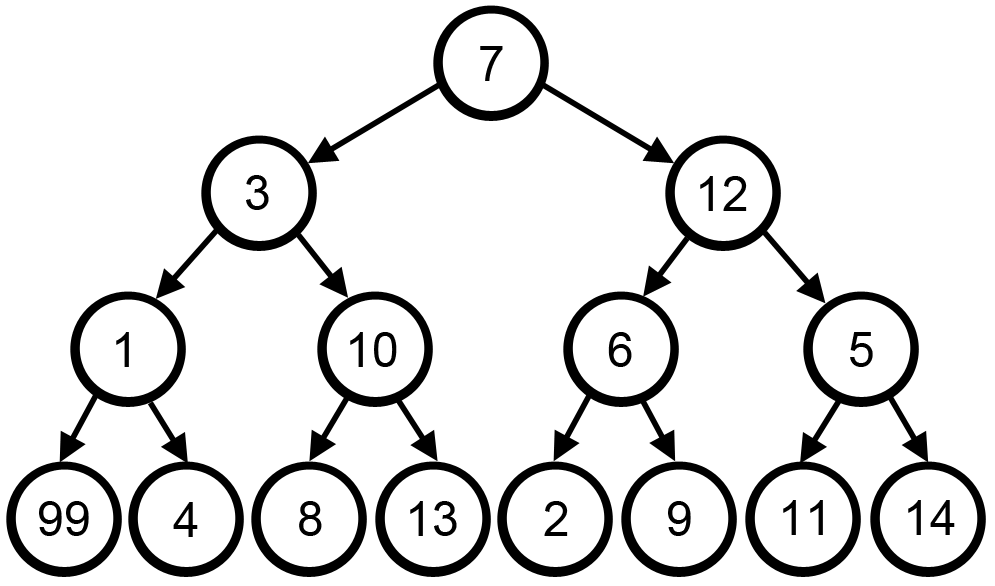
\includegraphics[width=7cm, height=7cm, keepaspectratio]{images/solving_2.png}}
\only<2>{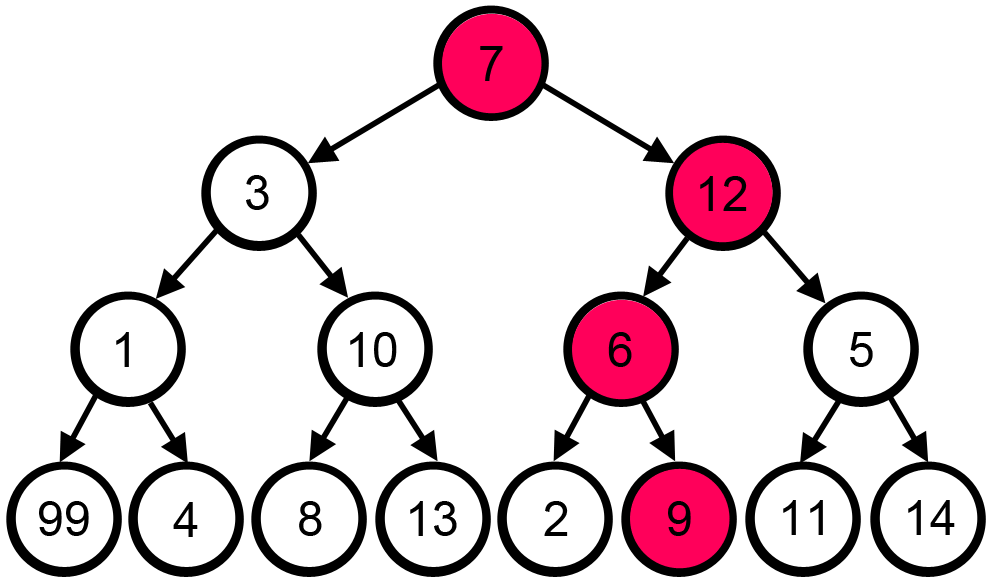
\includegraphics[width=7cm, height=7cm, keepaspectratio]{images/solving_3.png}}
\end{center}
\end{column}
\end{columns}
\end{frame}

\begin{frame}{Az $\varepsilon$-mohó stratégia}
\begin{columns}
\begin{column}{.5\textwidth}
Egy másik lehetőség, ha adott valószínűséggel az ügynök véletlen cselekvést hajt végre remélve, hogy ezzel elér egy olyan állapotba amelyhez nagy jutalom tartozik. A véletlen cselekvés a \textbf{felfedezés}, és végrehajtásának valószínűsége $\epsilon$.
\begin{center}
\begin{block}{$\varepsilon$-mohó cselekvés választás}
\[
A_{t}\leftarrow\begin{cases}
_{a\sim A}^{\underset{a}{argmax}Q(a)} & _{P=\varepsilon}^{P=1-\varepsilon}\end{cases}
\]
\end{block}
\end{center}
\end{column}
\begin{column}{.5\textwidth}
Az ügynök tehát $\varepsilon$ valószínűséggel véletlen cselekvést választ az ismeretlen, de nagyobb jutalom reményében. Ez a \textbf{felfedezés} művelete.\\
$\varepsilon$ valószínűséggel pedig a már ismert és a legnagyobb várható jutalommal járó cselekvést hajtja végre. Ez a \textbf{kizsákmányolás} művelete.
\begin{center}
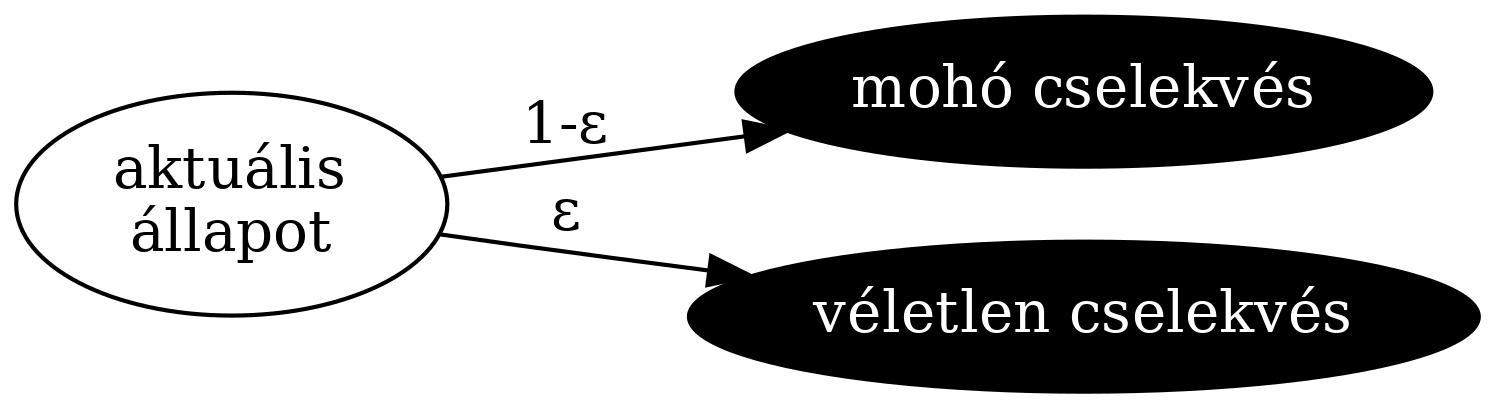
\includegraphics[width=7cm, height=6cm, keepaspectratio]{graphs/solving_1.png}
\end{center}
\end{column}
\end{columns}
\end{frame}

\begin{frame}{Példák}
A következő valós példák alkalmasak a felfedezés/kizsákmányolás dilemma bemutatására:
\begin{itemize}
	\item Étterem választás:
	\begin{itemize}
		\item Kizsákmányolás: elmész a kedvenc éttermedbe.
		\item Felfedezés: elmész egy új étterembe, hátha találsz egy jobbat mint a kedvenced.
	\end{itemize}
	\item Online hirdetés:
	\begin{itemize}
		\item Kizsákmányolás: a legjobb reklám megmutatása a felhasználónak.
		\item Felfedezés: egy új reklám megmutatása a felhasználónak, hátha tetszik neki.
	\end{itemize}
	\item Olajfúrás:
	\begin{itemize}
		\item Kizsákmányolás: Egy meglévő helyen fúrás az olajért.
		\item Felfedezés: Egy új helyen fúrás.
	\end{itemize}
	\item Klinikai kezelés:
	\begin{itemize}
		\item Kizsákmányolás: A bevált kezelés alkalmazása.
		\item Felfedezés: Új kezelés kipróbálása.
	\end{itemize}
\end{itemize}
\end{frame}

\begin{frame}{A rabló probléma}
\begin{columns}
\begin{column}{.5\textwidth}
A $k$-karú rabló problémája egy elméleti megerősítéses tanulás probléma. A játékos egy rablógépen játszik, amelynek $k$ karja van. Minden karhúzás után egy állandó eloszlásból választott jutalmat kap az ügynök. Az ügynök célja, hogy olyan politikát válasszon, ami az elvárt hozamot maximalizálja $1000$ cselekvés vagy \emph{időlépés} után.
\end{column}
\end{columns}
\end{frame}

\end{document}












